%----------
%   IMPORTANTE
%----------

% Esta plantilla está basada en las recomendaciones de la guía "Trabajo fin de Grado: Escribir el TFG", que encontrarás en http://uc3m.libguides.com/TFG/escribir
% contiene recomendaciones de la Biblioteca basadas principalmente en estilos APA e IEEE, pero debes seguir siempre las orientaciones de tu Tutor de TFG y la normativa de TFG para tu titulación.



% ESTA PLANTILLA ESTÁ BASADA EN EL ESTILO APA


%----------
%	CONFIGURACIÓN DEL DOCUMENTO
%----------

\documentclass[12pt]{report} % fuente a 12pt

% MÁRGENES: 2,5 cm sup. e inf.; 3 cm izdo. y dcho.xx
\usepackage[
a4paper,
vmargin=2cm,
hmargin=3cm
]{geometry}

% INTERLINEADO: Estrecho (6 ptos./interlineado 1,15) o Moderado (6 ptos./interlineado 1,5)
\renewcommand{\baselinestretch}{1.25}
\parskip=12pt

% DEFINICIÓN DE COLORES para portada y listados de código
\usepackage[table]{xcolor}
\definecolor{azulUC3M}{RGB}{0,0,102}
\definecolor{gray97}{gray}{.97}
\definecolor{gray75}{gray}{.75}
\definecolor{gray45}{gray}{.45}

%colors for hightlights
\usepackage{xcolor}
\usepackage{soul}
\newcommand{\highlight}[1]{\sethlcolor{yellow}\hl{#1}}
\newcommand{\question}[1]{\sethlcolor{red}\hl{QUESTION #1}}
\newcommand{\todo}[1]{\sethlcolor{green}\hl{TODO #1}}

% Soporte para GENERAR PDF/A --es importante de cara a su inclusión en e-Archivo porque es el formato óptimo de preservación y a la generación de metadatos, tal y como se describe en http://uc3m.libguides.com/ld.php?content_id=31389625. 

% En la plantilla incluimos el archivo OUTPUT.XMPDATA. Puedes descargar este archivo e incluir los metadatos que se incorporarán al archivo PDF cuando compiles el archivo memoria.tex. Después vuelve a subirlo a tu proyecto.  
\usepackage[a-1b]{pdfx}

% ENLACES
\usepackage{hyperref}
\hypersetup{colorlinks=true,
	linkcolor=black, % enlaces a partes del documento (p.e. índice) en color negro
	urlcolor=blue} % enlaces a recursos fuera del documento en azul

% EXPRESIONES MATEMÁTICAS
\usepackage{amsmath,amssymb,amsfonts,amsthm}

% Codificación caracteres
\usepackage{txfonts} 
\usepackage[T1]{fontenc}
\usepackage[utf8]{inputenc}

\usepackage[english]{babel} 
\AtBeginEnvironment{quote}{\small}

% diseño de PIE DE PÁGINA
\usepackage{fancyhdr}
\pagestyle{fancy}
\fancyhf{}
\renewcommand{\headrulewidth}{0pt}
\rfoot{\thepage}
\fancypagestyle{plain}{\pagestyle{fancy}}

% DISEÑO DE LOS TÍTULOS de las partes del trabajo (capítulos y epígrafes o subcapítulos)
\usepackage{titlesec}
\usepackage{titletoc}
\titleformat{\chapter}[block]
{\large\bfseries\filcenter}
{\thechapter.}
{5pt}
{\MakeUppercase}
{}
\titlespacing{\chapter}{0pt}{0pt}{*3}
\titlecontents{chapter}
[0pt]                                               
{}
{\contentsmargin{0pt}\thecontentslabel.\enspace\uppercase}
{\contentsmargin{0pt}\uppercase}                        
{\titlerule*[.7pc]{.}\contentspage}                 

\titleformat{\section}
{\bfseries}
{\thesection.}
{5pt}
{}
\titlecontents{section}
[5pt]                                               
{}
{\contentsmargin{0pt}\thecontentslabel.\enspace}
{\contentsmargin{0pt}}
{\titlerule*[.7pc]{.}\contentspage}

\titleformat{\subsection}
{\normalsize\bfseries}
{\thesubsection.}
{5pt}
{}
\titlecontents{subsection}
[10pt]                                               
{}
{\contentsmargin{0pt}                          
	\thecontentslabel.\enspace}
{\contentsmargin{0pt}}                        
{\titlerule*[.7pc]{.}\contentspage}  

% DISEÑO DE TABLAS y FIGURAS
\usepackage{multirow} % permite combinar celdas 
\usepackage{caption} % para personalizar el título de tablas y figuras
\usepackage{floatrow} % utilizamos este paquete y sus macros \ttabbox y \ffigbox para alinear los nombres de tablas y figuras de acuerdo con el estilo definido.
\usepackage{array} % con este paquete podemos definir en la siguiente línea un nuevo tipo de columna para tablas: ancho personalizado y contenido centrado
\newcolumntype{P}[1]{>{\centering\arraybackslash}p{#1}}
\DeclareCaptionFormat{upper}{#1#2\uppercase{#3}\par}
\usepackage{graphicx}
\usepackage{float}
\graphicspath{{images/}} % ruta a la carpeta de imágenes

% Diseño de tabla para ciencias sociales y humanidades


% Diseño de figuras para ciencias sociales y humanidades
\captionsetup[all]{
    justification=centering,
    singlelinecheck=true,
    labelfont=bf,
    textfont=it,
    font=small,
    skip=0pt
}
\floatsetup[all]{
    heightadjust=caption,
    footposition=bottom,
    font=small
}

% Configuración del pie de las figuras y tablas 
\captionsetup*[floatfoot]{
    footfont={small, up}
}

% NOTAS A PIE DE PÁGINA
\usepackage{chngcntr} % para numeración continua de las notas al pie
\counterwithout{footnote}{chapter}

% LISTADOS DE CÓDIGO
% soporte y estilo para listados de código. Más información en https://es.wikibooks.org/wiki/Manual_de_LaTeX/Listados_de_código/Listados_con_listings
\usepackage{listings}

% definimos un estilo de listings
\lstdefinestyle{estilo}{ frame=Ltb,
	framerule=0pt,
	aboveskip=0.5cm,
	framextopmargin=3pt,
	framexbottommargin=3pt,
	framexleftmargin=0.4cm,
	framesep=0pt,
	rulesep=.4pt,
	backgroundcolor=\color{gray97},
	rulesepcolor=\color{black},
	%
	basicstyle=\ttfamily\footnotesize,
	keywordstyle=\bfseries,
	stringstyle=\ttfamily,
	showstringspaces = false,
	commentstyle=\color{gray45},     
	%
	numbers=left,
	numbersep=15pt,
	numberstyle=\tiny,
	numberfirstline = false,
	breaklines=true,
	xleftmargin=\parindent
}

\captionsetup*[lstlisting]{font=small, labelsep=period}
% fijamos el estilo a utilizar 
\lstset{style=estilo}
\renewcommand{\lstlistingname}{\uppercase{Código}}


%BIBLIOGRAFÍA 

% CONFIGURACIÓN PARA LA BIBLIOGRAFÍA APA
\usepackage[style=apa, backend=biber, natbib=true, hyperref=true, uniquelist=false, sortcites]{biblatex}
\DeclareLanguageMapping{english}{english-apa}

% Para sustituir % por y o e
\makeatletter
\DefineBibliographyExtras{english}{%
  \setcounter{smartand}{1}%
  \let\lbx@finalnamedelim=\lbx@en@smartand
  \let\lbx@finallistdelim=\lbx@en@smartand
}

\makeatother


\addbibresource{referencias.bib} % llama al archivo referencias.bib en el que deberá estar la bibliografía utilizada


%-------------
%	DOCUMENTO
%-------------

% Dont split paragraphs between page breaks
\widowpenalties 1 10000
\raggedbottom


\begin{document}
\pagenumbering{roman} % Se utilizan cifras romanas en la numeración de las páginas previas al cuerpo del trabajo
	
%----------
%	PORTADA
%----------	
\begin{titlepage}
	\begin{sffamily}
	\color{azulUC3M}
	\begin{center}
		\begin{figure}[H] %incluimos el logotipo de la Universidad
			\makebox[\textwidth][c]{
\includegraphics[width=16cm]{logo_UC3M.png}}
		\end{figure}
		\vspace{2.5cm}
		\begin{Large}
			Grado Universitario...\\			
			 2020-2021\\ %Indica el curso académico
			\vspace{2cm}		
			\textsl{Trabajo Fin de Grado}
			\bigskip
			
		\end{Large}
		 	{\Huge ``Título del trabajo''}\\
		 	\vspace*{0.5cm}
	 		\rule{10.5cm}{0.1mm}\\
			\vspace*{0.9cm}
			{\LARGE Nombre Apellido1 Apellido2}\\ 
			\vspace*{1cm}
		\begin{Large}
			Tutor/es\\
			Nombre Apellido1 Apellido2\\
			Nombre Apellido1 Apellido2\\
			Lugar y fecha de presentación prevista\\
		\end{Large}
	\end{center}
	\vfill
	\color{black}
	% SI NUESTRO TRABAJO SE VA A PUBLICAR CON UNA LICENCIA CREATIVE COMMONS, INCLUIR ESTAS LÍNEAS. ES LA OPCIÓN RECOMENDADA.
	
\includegraphics[width=4.2cm]{creativecommons.png}\\ %incluimos el logotipo de Creative Commons
	Esta obra se encuentra sujeta a la licencia Creative Commons \textbf{Reconocimiento - No Comercial - Sin Obra Derivada}
	\end{sffamily}
\end{titlepage}

\newpage %página en blanco o de cortesía
\thispagestyle{empty}
\mbox{}

%----------
%	RESUMEN Y PALABRAS CLAVE
%----------	
\renewcommand\abstractname{\large\bfseries\filcenter\uppercase{Resumen}}
\begin{abstract}
\thispagestyle{plain}
\setcounter{page}{3}
	
	% ESCRIBIR EL RESUMEN AQUÍ
	
	\textbf{Palabras clave:}
	% Escribir las palabras clave aquí
	
	\vfill
\end{abstract}
	\newpage % página en blanco o de cortesía
	\thispagestyle{empty}
	\mbox{}


%----------
%	DEDICATORIA
%----------	
\chapter*{Dedicatoria} % \chapter* evita que aparezca en el índice

\setcounter{page}{5}
	
	% ESCRIBIR LA DEDICATORIA AQUÍ	
		
	\vfill
	
	\newpage % página en blanco o de cortesía
	\thispagestyle{empty}
	\mbox{}
	

%----------
%	ÍNDICES
%----------	

%--
% Índice general
%-
\tableofcontents
\thispagestyle{fancy}

\newpage % página en blanco o de cortesía
\thispagestyle{empty}

% Índice de figuras. Si no se incluyen, comenta las líneas siguientes
%-
\listoffigures
\thispagestyle{fancy}

\newpage % página en blanco o de cortesía
\thispagestyle{empty}
\mbox{}

%--
% Índice de tablas. Si no se incluyen, comenta las líneas siguientes
%-
\listoftables
\thispagestyle{fancy}

\newpage % página en blanco o de cortesía
\thispagestyle{empty}
\mbox{}


%----------
%	MEMORIA
%----------	
\clearpage
\pagenumbering{arabic} % numeración con números arábigos para el resto de la memoria.	

%--
% Report
%-------------------------------------
\chapter{Introduction}

\todo{introduction saying what we are going to do}

\section{Initial parameters}

For our case the initial parameters that we will be using will be the ones given in the Figure \ref{fig:introduction:initial_parameters}.

\begin{figure}[htbp]
    \centering
    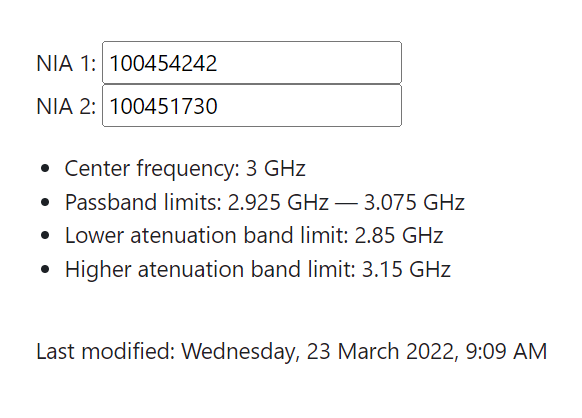
\includegraphics[width=0.65\textwidth]{introduction/initial_parameters_calculator.png}
    \caption{Initial parameters for our case study.}
    \label{fig:introduction:initial_parameters}
\end{figure}

\todo{add a section with the constants used}


%-------------------------------------
\chapter{Previous Work}
\section{Substrate Selection}

For the circuit design we will be using a substrate with a microstrip structure with two possible dielectric thickness of $h = 0.508 mm$ or $h = 1.27 mm$ and a thick copper metallization of $t = 17 \mu m$. For the substrate type the different configuration are seen in the Table \ref{tab:previous_work:substrate_types}.

\begin{table}[htbp]
    \centering
    \caption{Substrate types}
    \label{tab:previous_work:substrate_types}
    \begin{tabular}{@{}llll@{}}
    Material & Relative permittivity ($\varepsilon_r$) & Loss tangent ($\tan \delta$) & Cost per area \\
    Fiberglass (FR4) & 4.7 & 0.01 & $\times 1$ \\
    RT/Duroid 5880 & 2.2 & 0.009 & $\times 10$ \\
    RT/Duroid 6006 & 6.15 & 0.0027 & $\times 10$ \\
    RT/Duroid 6010.2LM & 10.2 & 0.0023 & $\times 10$ \\
    \end{tabular}
\end{table}

\subsection{Substrate type}

As we can see in table \ref{tab:previous_work:substrate_types}, the \textit{Fiberglass (FR4)} has a really high loss tangent $\tan \delta$. Even though it is the cheapest, we have decided to use another substrate that has a better $\tan \delta$ in order to improve our amplifier. For the choices, we can only choose the \textit{RT/Duroid 6006} or the \textit{RT/Duroid 6010.2LM} as the \textit{RT/Duroid 5880} as almost the same $\tan \delta$ as \textit{Fiberglass (FR4)}.

Comparing the  \textit{RT/Duroid 6006} and the \textit{RT/Duroid 6010.2LM}, we can observe that they have the same price so we will go with the one with the lowest $\tan \delta$. That is as we want to reduce the losses at maximum. So let's study the \textit{RT/Duroid 6010.2LM}. 

If we use the values given the in the Table \ref{tab:previous_work:substrate_types} for the \textit{RT/Duroid 6010.2LM} and the AWR TXLine tool, we get a microstrip width of $w = 0.458 $ when the dielectric thickness of $h = 0.508 mm $ for a $Z = 50 \Omega$ (See Figure \ref{fig:previous_work:duroid_6010.2lm_h_1_27_mm_50_ohm}). On the other hand, if we use a $h = 1.27 mm$ for a $Z = 50 \Omega$, we get a microstrip width of $w = 1.17 mm$ which is larger (See Figure \ref{fig:previous_work:duroid_6010.2lm_h_1_27_mm_50_ohm}.

\begin{figure}[htbp]
    \centering
    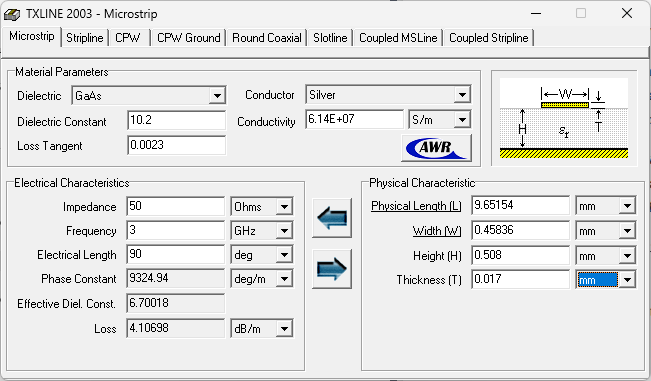
\includegraphics[width=\textwidth]{images/previous_work/txline_tool_duroid_6010.2lm_h_0_508_mm_50_ohm.png}
    \caption{Width $w = 0.458 mm$ for RT/Duroid 6010.2LM with $h = 0.508 mm$ and a $Z = 50 \Omega$}
    \label{fig:previous_work:duroid_6010.2lm_h_0_508_mm_50_ohm}
\end{figure}

\begin{figure}[htbp]
    \centering
    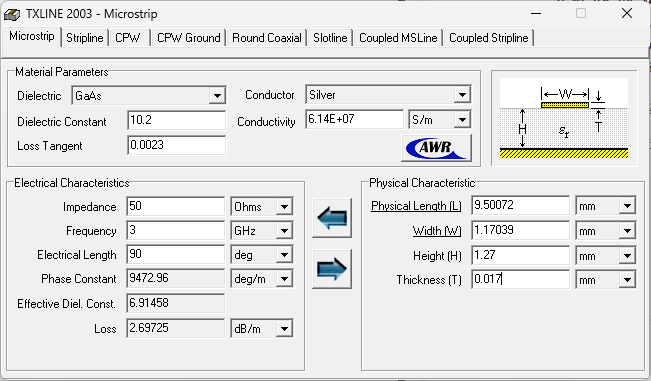
\includegraphics[width=\textwidth]{images/previous_work/txline_tool_duroid_6010.2lm_h_1_27_mm_50_ohm.png}
    \caption{Width $w = 1.17 mm$ for RT/Duroid 6010.2LM with $h = 1.27 mm$ and a $Z = 50 \Omega$}
    \label{fig:previous_work:duroid_6010.2lm_h_1_27_mm_50_ohm}
\end{figure}

Considering that the width of each line must be no less than $200 \mu m$, both lines would work perfectly fine at $Z = 50 \Omega$. However, as we are designing a circuit where we might need different values of $Z$, we will see if they still work for for example $Z = 100 \Omega$.

Using the \textit{RT/Duroid 6010.2LM} with  a dielectric thickness of $h = 1.27 mm$ for $Z = 100 \Omega$ we get a microstrip width of $w = 0.144mm$ (See Figure \ref{fig:previous_work:duroid_6010.2lm_h_1_27_mm_100_ohm}). As the width needed, is smaller than the one required, this substrate it is not the most recommended.

\begin{figure}[htbp]
    \centering
    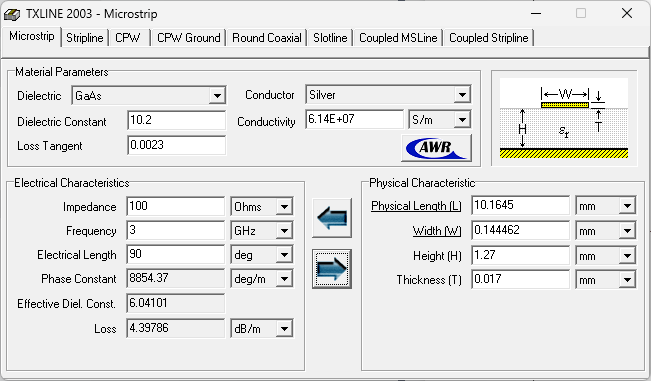
\includegraphics[width=\textwidth]{images/previous_work/txline_tool_duroid_6010.2lm_h_1_27_mm_100_ohm.png}
    \caption{Width $w = 0.144 mm$ for RT/Duroid 6010.2LM with $h = 1.27 mm$ and a $Z = 100 \Omega$}
    \label{fig:previous_work:duroid_6010.2lm_h_1_27_mm_100_ohm}
\end{figure}

Due to that inconvenience, let's study the substrate \textit{RT/Duroid 6006}. For this substrate with a $h = 1.27 mm$ and a $Z = 100 \Omega$, we get a width of $w = 0.343 mm$ (See Figure \ref{fig:previous_work:duroid_6006_h_1_27_mm_100_ohm}). This width is much better than the \textit{RT/Duroid 6010.2LM} with the $200 \mu m$ minimum width constraint as we have more room to design our circuit. Therefore, \highlight{we will be using the \textit{RT/Duroid 6006}}.

\begin{figure}[htbp]
    \centering
    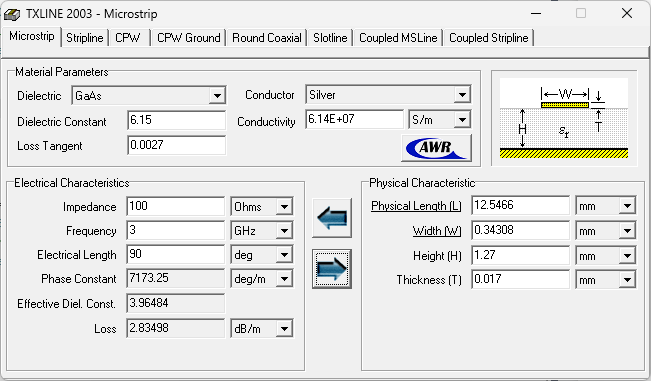
\includegraphics[width=\textwidth]{images/previous_work/txline_tool_duroid_6006_h_1_27_mm_100_ohm.png}
    \caption{Width $w = 0.343 mm$ for RT/Duroid 6006 with $h = 1.27 mm$ and a $Z = 100 \Omega$}
    \label{fig:previous_work:duroid_6006_h_1_27_mm_100_ohm}
\end{figure}

\subsection{Substrate dielectric thickness}

For the dielectric thickness, we can see in Figure \ref{fig:previous_work:duroid_6006_h_0_508_mm_100_ohm} that for the \textit{RT/Duroid 6006} with a $h = 0.508 mm$ and a $Z = 100 \Omega$, we get a width of $w = 0.128$. As stated before, that does not check the constraint of a minimum width of $w = 0.2 mm$. Because of that \highlight{we will select a dielectric thickness of $h = 1.27 mm$}.

\begin{figure}[htbp]
    \centering
    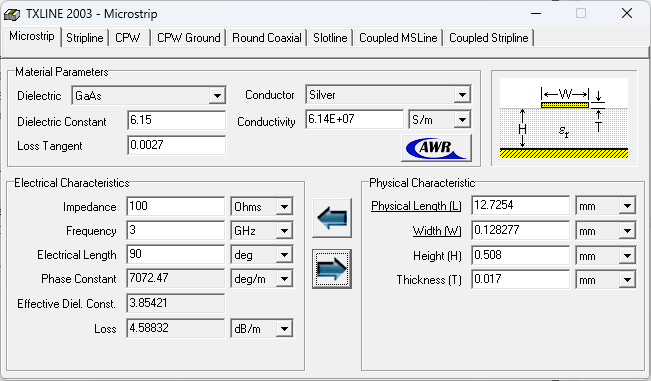
\includegraphics[width=\textwidth]{images/previous_work/txline_tool_duroid_6006_h_0_508_mm_100_ohm.png}
    \caption{Width $w = 0.128 mm$ for RT/Duroid 6006 with $h = 0.508 mm$ and a $Z = 100 \Omega$}
    \label{fig:previous_work:duroid_6006_h_0_508_mm_100_ohm}
\end{figure}

\subsection{Final substrate selection}

For the substrate, we will select the \textit{RT/Duroid 6006} as it is the best one for the same price that fits the constraints required. For the dielectric thickness, we will use a $h = 1.27 mm$ for the very same reason. Choosing this dielectric will make our circuit as small as possible while keeping the losses at minimum. The price is not a concern as the \textit{Fiberglass (FR4)}, even though it is the cheapest, we decided to discarded due to its really high $\tan \delta$. And among the rest of the substrates, the price is the same.

Finally, in the Figure \ref{fig:previous_work:duroid_6006_h_1_27_mm_50_ohm}, we can see the calculations of the final width of $w = 1.85 mm$ for a characteristic impedance of $Z_{0} = 50 \Omega$ and a dielectric thickness of $h = 1.27 mm$. As we can see, the width is bigger than $w = 200 \mu m$, therefore it checks the constraints and it will be the one we will be using further on.

\todo{maybe study the length a the lambda/4, i dont know how to do it (Andres)}

\begin{figure}[htbp]
    \centering
    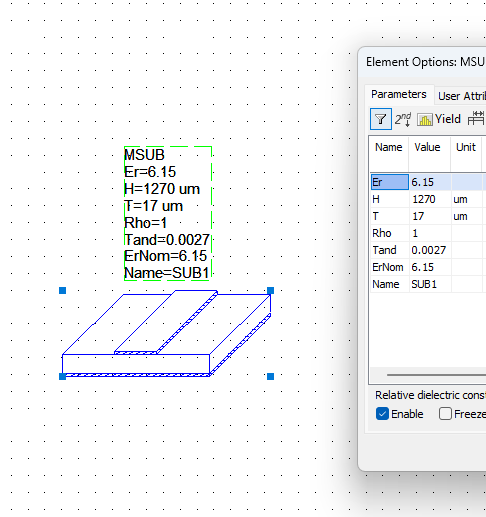
\includegraphics[width=0.75\textwidth]{images/previous_work/final_substrate_duroid_6006_h_1_27_mm.png}
    \caption{Final substrate selection}
    \label{fig:previous_work:final_substrate}
\end{figure}

\begin{figure}[htbp]
    \centering
    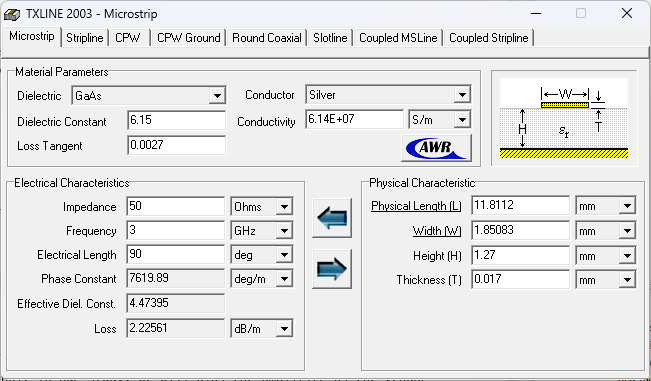
\includegraphics[width=\textwidth]{images/previous_work/txline_tool_duroid_6006_h_1_27_mm_50_ohm.png}
    \caption{Width $w = 1.85 mm$ for RT/Duroid 6006 with $h = 1.27 mm$ and a $Z = 50 \Omega$}
    \label{fig:previous_work:duroid_6006_h_1_27_mm_50_ohm}
\end{figure}

\chapter{Design of the Circuit Elements}
\section{First Stage: Simple Amplifier}

For the amplifier, we will be using the GVA83+, which is a wide band amplifier for a dynamic range of applications. In order for an amplifier to work, it needs to be supplied a DC power in order for it to perform the amplification of our signal. In our study, we will bias the amplifier as the vendor recommends, see Figure \ref{fig:design_circuit_elements:gva83+_bias_configuration}. 

\begin{figure}[htbp]
    \centering
    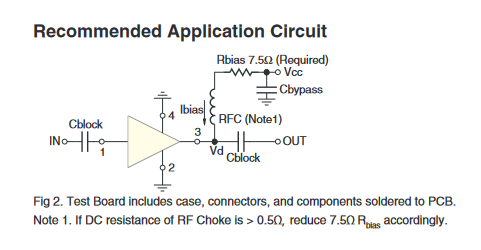
\includegraphics[width=\textwidth]{images/design_circuit_elements/gva83+_bias_configuration.png}
    \caption{Bias network of the GVa83+ Amplifier recommended by the vendor}
    \label{fig:design_circuit_elements:gva83+_bias_configuration}
\end{figure}

\subsection{Analysis of the Bias Network (Figure \ref{fig:design_circuit_elements:gva83+_bias_configuration}) at f = 0 GHz and f = 3 GHz}

When $f = 0 GHz$, we can observe that the impedance of the capacitors $Z_{C} = \frac{1}{j \cdot 2 \cdot \pi \cdot f \cdot C} \xrightarrow{} \infty$ when $f \xrightarrow{} 0$ acting as an open circuit. On the other hand, the impedance of the inductor $Z_{L} = j \cdot 2 \cdot \pi \cdot f \cdot L \xrightarrow{} 0$ when $f \xrightarrow{} 0$ acting as a short circuit. Taking those points into account, we get that the circuit can be summarized as seen in Figure \ref{fig:design_circuit_elements:gva83+_bias_f_0_ghz} when $f = 0 GHz$. Since the output is not connected to the input, then the circuit will not work at very low frequencies. However, we can calculate the current flowing through the inductor as it is a short circuit now, and that current will be the one in charge of powering the amplifier. In this case $I_{bias} = \frac{V_{CC}}{R_{bias}}$ .

\begin{figure}[htbp]
    \centering
    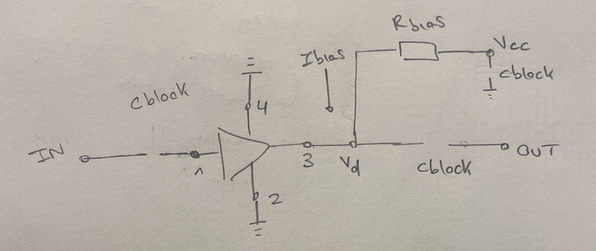
\includegraphics[width=\textwidth]{images/design_circuit_elements/gva83+_bias_f_0_ghz.png}
    \caption{Bias network of the GVa83+ Amplifier at $f = 0 GHz$}
    \label{fig:design_circuit_elements:gva83+_bias_f_0_ghz}
\end{figure}

On the other hand, if we study the circuit at the designed frequency $f = 3 GHz$; the capacitors act as a short circuit and the inductor act as an open circuit. That way, the branch required to bias the amplifier is "disconnected" per say (See Figure \ref{fig:design_circuit_elements:gva83+_bias_f_3_ghz}) and the gain of the amplifier is $G = Av = s_{21}$.

\begin{figure}[htbp]
    \centering
    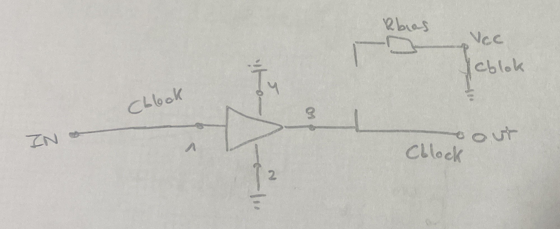
\includegraphics[width=\textwidth]{images/design_circuit_elements/gva83+_bias_f_3_ghz.png}
    \caption{Bias network of the GVa83+ Amplifier at $f = 3 GHz$}
    \label{fig:design_circuit_elements:gva83+_bias_f_3_ghz}
\end{figure}

\subsection{Analysis of the Bias Network (Figure \ref{fig:design_circuit_elements:gva83+_bias_configuration}) with the Transmission Line at f = 0 GHz and f = 3 GHz}

The analysis of the proposed Bias Network with the Transmission Line (TL) (see Figure \ref{fig:design_circuit_elements:gva83+_bias_transmission_line}) is really similar to the one proposed by the vendor (see Figure \ref{fig:design_circuit_elements:gva83+_bias_configuration}). The only differences are that we are using a TL instead of an inductor and the bypass capacitor now it is in parallel with the TL.

At $f = 0 GHz$, the capacitors act as open circuits and the TL acts as a short circuit. Again, since the output is not connected to the amplifier, the circuit does not work as previously stated. On the other hand, at $f = 3 GHz$, the capacitors act as a short circuit and the TL acts as an open circuit as before. The gain of the circuit is still the same as before $G = Av = s{21}$.

In order to calculate the length of the TL in order to function as the inductor, we need to get the highest possible value of the characteristic impedance ($Z_0$). For this we have used the AWR TXLine tool and we got a length of $l = 12.692 mm$ with a characteristic impedance of $Z_0 = 130.62 \Omega$ (see Figure \ref{fig:design_circuit_elements:txline_tool_bias_network_amplifier_transmission_line}). Keep in mind that we have used the minimum width available $w = 200 \mu m$ in order to make it as small as possible. The reasoning for getting the maximum $Z_0$ is because that way, the TL will behave like an open circuit for high frequencies and like a short circuit for low frequencies.

\question{is this explanation correct for the max $Z_0$ to get the length? is the calculation correct}

\begin{figure}[htbp]
    \centering
    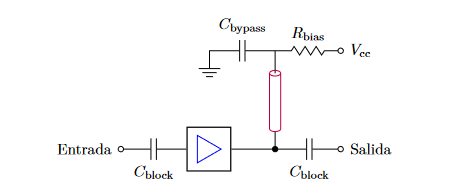
\includegraphics[width=\textwidth]{images/design_circuit_elements/gva83+_bias_transmission_line.png}
    \caption{Proposed Bias Network of the GVa83+ Amplifier with a TL}
    \label{fig:design_circuit_elements:gva83+_bias_transmission_line}
\end{figure}

\begin{figure}[htbp]
    \centering
    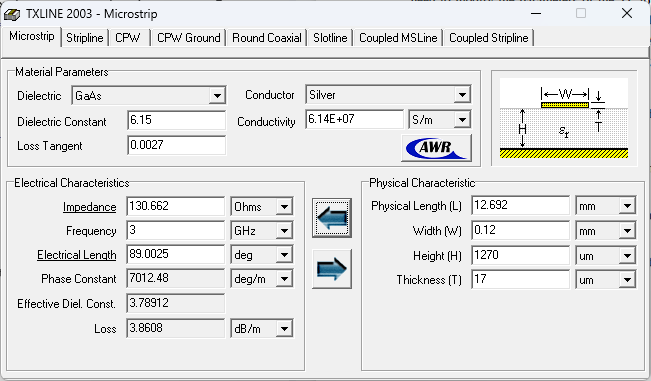
\includegraphics[width=\textwidth]{images/design_circuit_elements/txline_tool_bias_network_amplifier_transmission_line.png}
    \caption{Length and $Z_0$ calculations of the TL of the Bias Network}
    \label{fig:design_circuit_elements:txline_tool_bias_network_amplifier_transmission_line}
\end{figure}

\question{We want a $Z_0$ as high as possible to make the TL the shortest no?}

\section{GVA-83+ respone}
 
\subsection{Scattering parameters at f = 3 GHz}

In our case, with a working frequency of f = 3 GHz (see Figure \ref{fig:introduction:initial_parameters}) and for the nominal temparture and bias conditions ($V_{CC} = 5V, R_{bias} = 7.5 \Omega$), we get the following scattering parameters:

\[
[S] = \begin{bmatrix}
s_{11} = -16.87 \ dB & \quad s_{12} = -25.06 \ dB \\
s_{21} = 15.34 \ dB & \quad s_{22} = -10.68 \ dB \\
\end{bmatrix}
\]

Where:
\begin{align*}
s_{11} & : \text{Input Return Loss} \\
s_{12} & : \text{Isolation} \\
s_{21} & : \text{Gain} \\
s_{22} & : \text{Output Return Loss}
\end{align*}

Note: this parameters are for the frequency $f = 2.9 GHz$ (see Figure \ref{fig:design_circuit_elements:scattering_parameters_datasheet}). However, that frequency is really close to our working frequency of $f = 3 GHz$ so there will be almost the same.

\begin{figure}[htbp]
    \centering
    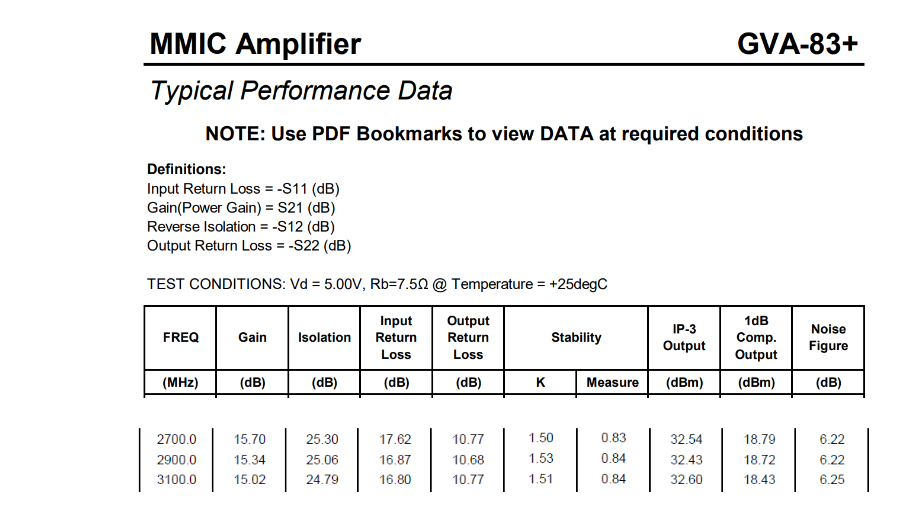
\includegraphics[width=\textwidth]{images/design_circuit_elements/scattering_parameters_datasheet.png}
    \caption{Scattering Parameters from the GVA-83+ datasheet}
    \label{fig:design_circuit_elements:scattering_parameters_datasheet}
\end{figure}

\subsection{Gain of each amplifier stage and the full two-stage network}
\label{subsec:gain_each_amplifier_and_full_two_stage}

The gain of just one amplifier is the scattering parameter $s_{21}$, so in our case the gain is $G = S{21} = 15.34 \ dB$. As the first stage and the second stage have just one amplifier, the gain of both of the will be the same of $G = 15.34 \ dB$. That is because the second stage behaves like a isolated amplifier with respect to the first stage.

For the full network, the gain of the whole circuit will be the product of both amplifiers as they are isolated to each other. That is the total gain will be $G_T = s_{21}^2$, so in dB it is \highlight{$G_T = 2 \cdot s_{21} (in \ dB) = 2 * 15.34 = 30.60 \ dB$}.

\subsection{Representation of the wide band S parameters}

In the Figure \ref{fig:design_circuit_elements:graph_amplifier}, we can see the scattering parameters at our working frequency $f = 3 GHz$. If we take a look at each parameter, we can clearly see that they are almost the same values as the ones we obtained from the datasheet (see Figure \ref{fig:design_circuit_elements:scattering_parameters_datasheet}).

\begin{figure}[htbp]
    \centering
    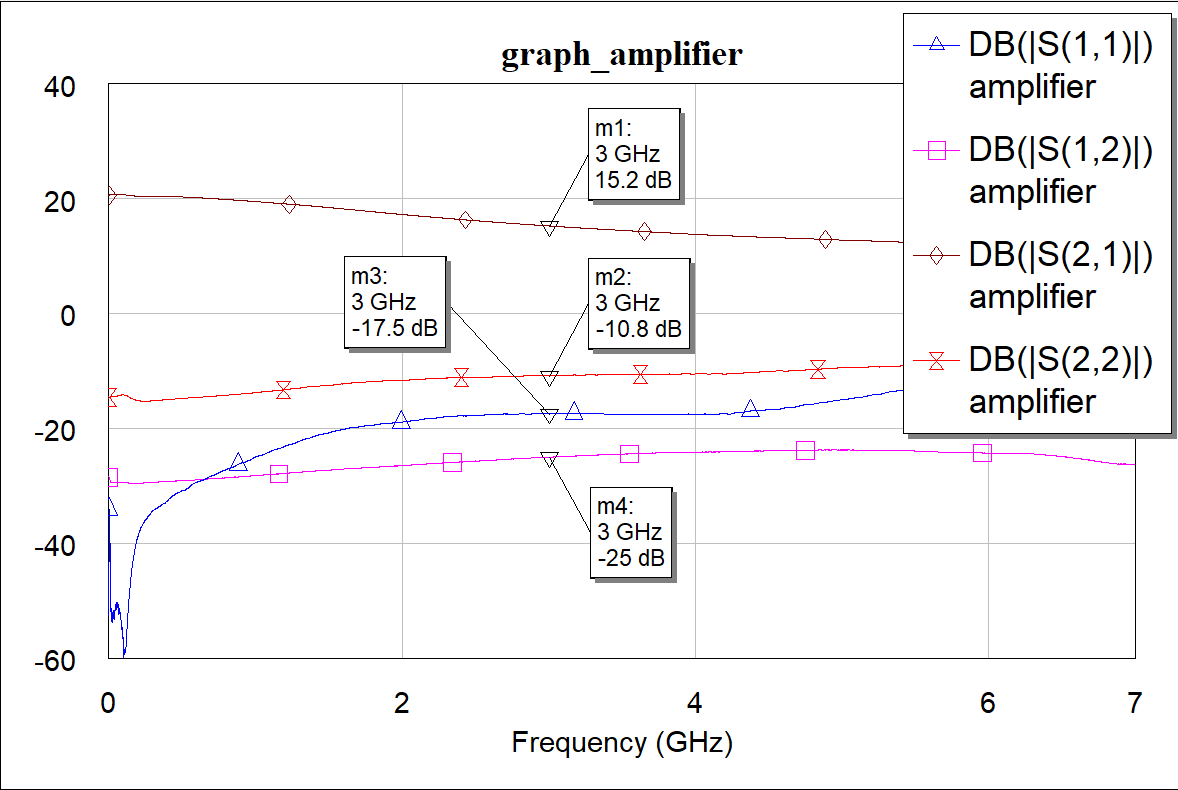
\includegraphics[width=\textwidth]{images/design_circuit_elements/graph_amplifier.png}
    \caption{AWR Graph of the GVA83+ Amplifier}
    \label{fig:design_circuit_elements:graph_amplifier}
\end{figure}

\section{Second Stage: Balanced Amplifier}

The second amplifier will be a balanced amplifier, that is a amplifier that first divides the signal into 2 signals and amplifies them separately. The idea with this amplifier, is to apply a phase shift to the signals of 180 degrees and them join them again at the end. With this configuration, as we are adding to signals that where shifted 180 degrees, any noise that we get in the amplifiers will be cancelled out resulting in a much cleaner signal.

For our case, we will have 3 different configurations depending on the order of the amplification and the phase shift. The configurations are described in Figure \ref{fig:design_circuit_elements:configurations_balanced_stage}. So let's get started and start by studying the different configurations.

Note: that for all of the configurations we will consider ideal Wilkinson combiners / dividers and a reference impedance of $Z_0 = 50 \Omega$. And we will be using the following scattering parameters:

For the Wilkinson we will be using: 

\[
[S_W] = \frac{-j}{\sqrt{2}} \* \begin{bmatrix}
0 & \quad 1 & \quad 1 \\
1 & \quad 0 & \quad 0 \\
1 & \quad 0 & \quad 0 \\
\end{bmatrix}
\]

For the amplifier:

\[
[S_A] = \begin{bmatrix}
s_{11A} & \quad s_{12A} \\
s_{21A} & \quad s_{22A} \\
\end{bmatrix}
\]

And finally for the phase shifter:

\[
[S_{\phi}] = \begin{bmatrix}
0 & \quad e^{-j \* \phi} \\
e^{-j \* \phi} & \quad 0 \\
\end{bmatrix}
\]

\begin{figure}[htbp]
    \centering
    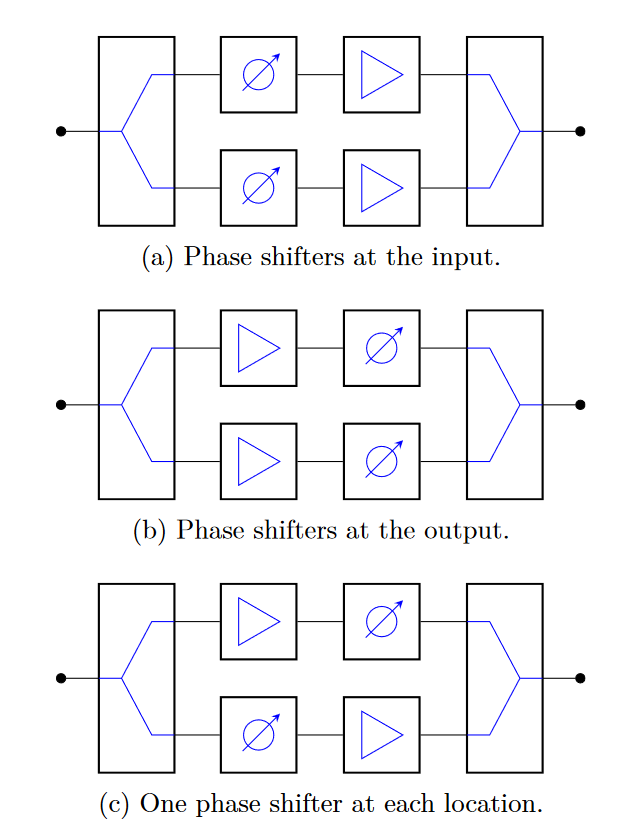
\includegraphics[width=\textwidth]{images/design_circuit_elements/configurations_balanced_stage.png}
    \caption{3 different configurations for the Balanced Stage}
    \label{fig:design_circuit_elements:configurations_balanced_stage}
\end{figure}

\subsection{S matrix for configuration (a) of Figure \ref{fig:design_circuit_elements:configurations_balanced_stage}}

For the first configuration, we get the following scattering parameters:

\[
[S] = \begin{bmatrix}
- s_{11A} \* e^{-2 \* j \* \phi} & \quad - s_{21A} \* e^{- j \* \phi} \\
- s_{21A} \* e^{- j \* \phi} & \quad - s_{22A} \\
\end{bmatrix}
\]

Note: that $s_{21} = s_{12}$ as the S matrix is reciprocal.

\subsection{S matrix for configuration (b) of Figure \ref{fig:design_circuit_elements:configurations_balanced_stage}}

For the second configuration, we get the following scattering parameters:

\[
[S] = \begin{bmatrix}
- s_{11A} & \quad - s_{21A} \* e^{- j \* \phi} \\
- s_{21A} \* e^{- j \* \phi} & \quad - s_{22A} \* e^{-2 \* j \* \phi} \\
\end{bmatrix}
\]

Note: that $s_{21} = s_{12}$ as the S matrix is reciprocal.

\subsection{S matrix for configuration (c) of Figure \ref{fig:design_circuit_elements:configurations_balanced_stage}}

Finally, for the last configuration, we get the following scattering parameters:

\[
[S] = \begin{bmatrix}
- \frac{s_{11A}}{2} \* (1 + e^{-2 \* j \* \phi}) & \quad - s_{21A} \* e^{- j \* \phi} \\
- s_{21A} \* e^{- j \* \phi} & \quad - \frac{s_{22A}}{2} \* (1 + e^{-2 \* j \* \phi}) \\
\end{bmatrix}
\]

Note: that $s_{21} = s_{12}$ as the S matrix is reciprocal.

\subsection{Comparison between the different configuration of Figure \ref{fig:design_circuit_elements:configurations_balanced_stage} and the simple amplifier}

Now that we have the 3 different S matrices, we can observe that they have the same transmission coefficients $s_{21} = s_{12} = - s_{21A} \* e^{- j \* \phi}$. That means that they will transmit the same power to the load. This makes sense as the only thing that differs between the configurations is the order of the components, but they are still the same.

On the other hand, if we consider the reflection coefficients ($s_{11}$ and $s_{22}$), we can see that they differ from one configuration to another. In order to see which configuration is best, we want the lowest reflection coefficients in order to have the least amount of power reflected as possible. In the first 2 configurations we can see that either $s_{11}$ or $s_{22}$ cannot be 0 (as they are not symmetrical), which means that in this two configuration we will have always some loss.

However, if we take a look at the last configuration we can see that if we apply a certain phase shift $\phi$, where $e^{- j \* \phi} = -1$, both coefficients become 0. Thus making the amplifier perfectly matchable without having any reflection. And for this very reason, the third configuration is best as we can achieve no reflection.

\subsection{Optimal phase shift}

As stated before, in order to have the (c) configuration to behave without losses, we need to make that $- \frac{s_{11A}}{2} \* (1 + e^{-2 \* j \* \phi}) = 0$. In order to do that, let's solve for $\phi$:

\begin{align*}
- \frac{s_{11a}}{2} (1 + e^{-2j\phi}) &= 0 \\
\rightarrow (1 + e^{-2j\phi}) &= 0 \\
\rightarrow e^{-2j\phi} &= -1 \\
\rightarrow \phi &= \frac{\pi}{2}
\end{align*}

So the optimal phase shift for the configuration (c) is $\phi = \frac{\pi}{2}$.

\subsection{Relationship between the output power at each branch of the balanced stage, and the total power at the output of the full balanced stage}

As shown previously in the Subsection \ref{subsec:gain_each_amplifier_and_full_two_stage},

\question{do i have to put the same of the section? or what?}

\section{Band Pass Filter}

\subsection{Filter order from the bandwidth, in-band return loss and the minimum attenuation at the stop bands}

Given the following values in the Figure \ref{fig:introduction:initial_parameters}:

\begin{align*}
\text{Center frequency} & : f_0 = 3 GHz\\
\text{Pass band lower limit} & : f_{p1} = 2.925 GHz\\
\text{Pass band upper limit} & : f_{p2} = 3.075 GHz\\
\text{Lower attenuation band limit} & : f_{a1} = 2.85 GHz\\
\text{Upper attenuation band limit} & : f_{a2} = 3.15 GHz\\
\end{align*}

And also, we have a requirement of a minimum attenuation of 25 dB. Therefore, we will be choosing an attenuation of $\alpha_{a} = 30 dB$ to be sure that the filter works correctly. As we want the input losses to be bigger than $20 dB$ then:

\begin{align*}
s_{11} >= 30 dB \Rightarrow s_{11} &= 30 dB \\
s_{11} &= 10^{\frac{-30}{20}} = 0.032
\end{align*}

Now that we have the return loss, we can calculate the maximum transmission loss (or better said the maximum pass band attenuation). As we want our filter to be lossless, then $s_{11}^2 + s_{12}^2 = 1$. With this formula and the previous value we calculated, we can get the following:

\begin{align*}
\alpha_{p} &= - 20 \* \log_{10}(s_{12}) \\
&= \-20 \* \log_{10}(\sqrt{1 - s_{11}^2}) \\
&= \-20 \* \log_{10}(\sqrt{1 - 0.032^2}) \\
&= 4.35 dBm
\end{align*}

\question{is this right? as they are not in the same column? do we want to be lossless? it is the only way if can think of to calculate the max attenuation at the pass band}

\question{how to calculate the order, do we use Chevyshev?}

\subsection{Parameters of the frequency and impedance transforms}

\todo{and a lot more todo, but how?}

\section{Directional Coupler}

In order to measure the signal and check the correct functionality, we will be using a directional coupler. Let's start with the study of the element.

\subsection{Electrical length and even and odd characteristic impedances of the couple-line section}

According to the requirements of the system, the power at the monitor port must be 20 dB below the main line. That means that the coupling of the directional amplifier must be $C_{dB} = 20 dB$.

\begin{align*}
C &= 10^{\frac{- C_{dB}}{10}} \\
&= 10^{\frac{- 20}{10}} \\
&= 0.1 \\
\end{align*}

Now, in order to calculate the characteristic impedances of the even and odd modes, first we will assume an electrical length of $\lambda / 4$ or the same as $90 \deg$. That means that the coupler will be a symmetric coupler with a $90 \deg$ phase shift between the transmitted and the coupled port,

\question{is this a symmetric coupler no?}

Given a electrical length of $\lambda / 4$, then we can use the following formulas to calculate the characteristic impedances of the even and odd modes, for the even mode we get:

\begin{align*}
Z_{0, even} &= Z_{0} \* \sqrt{\frac{1 + C}{1 - C}} \\
&= 55.28 \Omega \\
\end{align*}

And for the odd mode:

\begin{align*}
Z_{0, odd} &= Z_{0} \* \sqrt{\frac{1 - C}{1 + C}} \\
&= 45.23 \Omega \\
\end{align*}

\question{is this right? the calculation for Z0, i got it from here}
\url{http://www.ittc.ku.edu/~jstiles/723/handouts/section_7_6_Coupled_Line_Couplers_package.pdf}

\subsection{Connection of the coupler}

For this coupler, the main objective is to transmit the whole power entering from the input to the transmitted and coupled ports. For this case, we want the following scattering parameter matrix:

\[
S = \begin{bmatrix}
0 & \alpha & j \* \beta & 0 \\
\alpha & 0 & 0 & j \* \beta \\
j \* \beta & 0 & 0 & \alpha \\
0 & j \* \beta & \alpha & 0 \\
\end{bmatrix}
\]

\question{is this matrix ok? port 2 is the coupled}

Where:
\begin{align*}
& \text{We assume an isolation of $I = \infty \ dB$}  \\
& \text{Port 1 is the input port} \\
& \text{Port 2 is the coupled port} \\
& \text{Port 3 is the transmission port} \\
& \text{Port 4 is the isolated port} \\
\end{align*}

Usually for a directed port, you want that the isolated port is degenerated with respect to the other 3. Therefore, we will be loading it with a matched load, that is equal to the characteristic impedance of $Z_0 = 50 \Omega$. You can see the final circuit for the directed coupler in Figure \ref{fig:design_circuit_elements:directional_coupler_ideal_circuit}.

\begin{figure}[htbp]
    \centering
    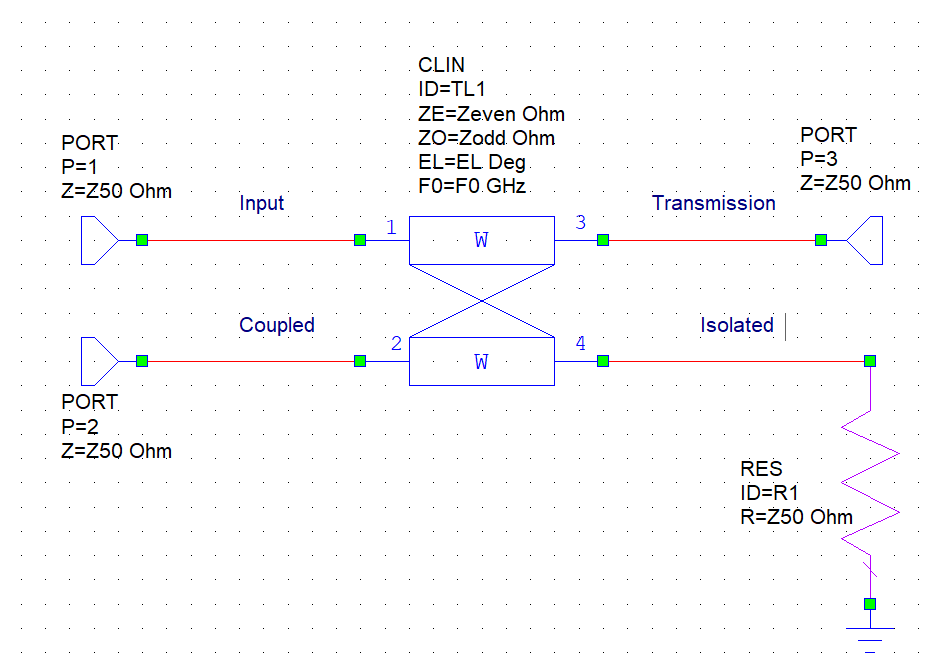
\includegraphics[width=\textwidth]{images/design_circuit_elements/directional_coupler_ideal_circuit.png}
    \caption{Ideal circuit for the directional coupler}
    \label{fig:design_circuit_elements:directional_coupler_ideal_circuit}
\end{figure}

If we simulate the circuit with AWR (see Figure \ref{fig:design_circuit_elements:directional_coupler_ideal_graph}), we can see that there is no reflection at the input port as the $s_{11} = -84 \ dB$, the coupling is $C = -20 \ dB$ as expected, and the rest of the power is directed to the transmission port.

\begin{figure}[htbp]
    \centering
    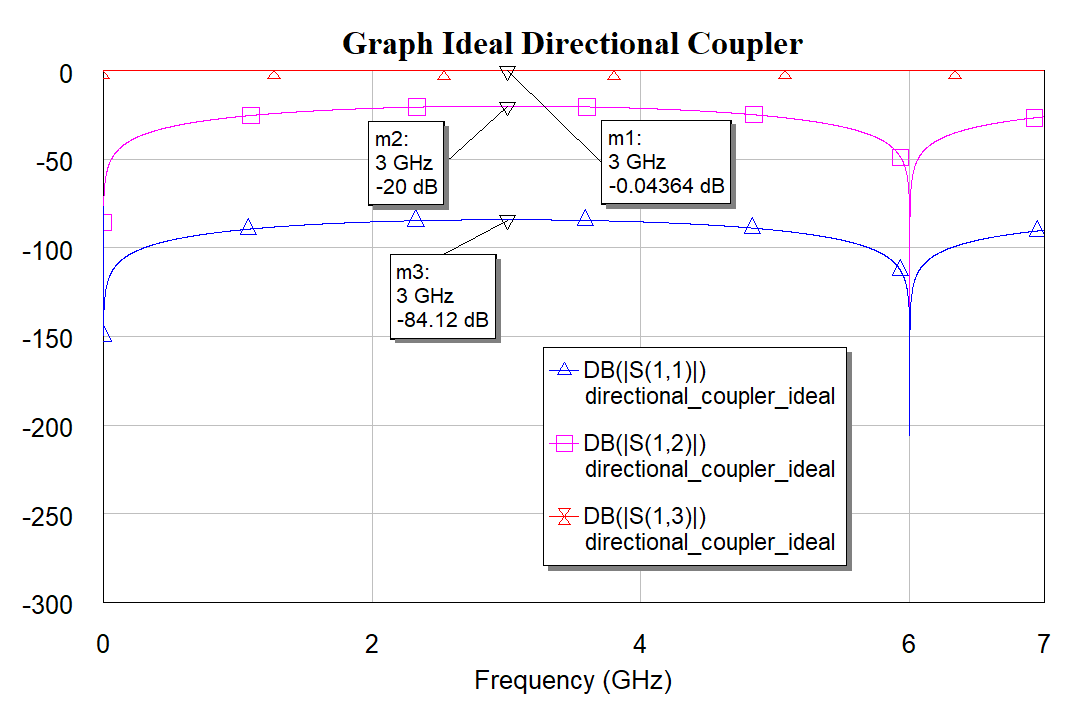
\includegraphics[width=\linewidth]{images//design_circuit_elements/directional_coupler_ideal_graph.png}
    \caption{Simulation of the ideal directed coupler of Figure \ref{fig:design_circuit_elements:directional_coupler_ideal_circuit}}
    \label{fig:design_circuit_elements:directional_coupler_ideal_graph}
\end{figure}

%-----------------------------------------------------------
\chapter{Design and Characterization of the Microstrip Elements}

\section{Wilkinson Power Divider / Combiner}

In order to divide the input signal from the simple amplifier into to equal signals and then join the signals together after they have been amplified in the second stage, we will be using a Wilkinson divider / combiner.

\subsection{Ideal Wilkinson Power Divider / Combiner}

First we have designed an ideal Wilkinson divider / combiner (see Figure \ref{fig:microstrip_elements:wilkinson_ideal_circuit}). We have used a resistance of $R = 2 \* Z_0 = 100 \Omega$ for the resistance between the two output ports. And also a characteristic impedance of the lines of $Z_{0,W} = \sqrt{2} \* Z_0 \ \Omega = 70.71 \ \Omega$.

\begin{figure}[htbp]
    \centering
    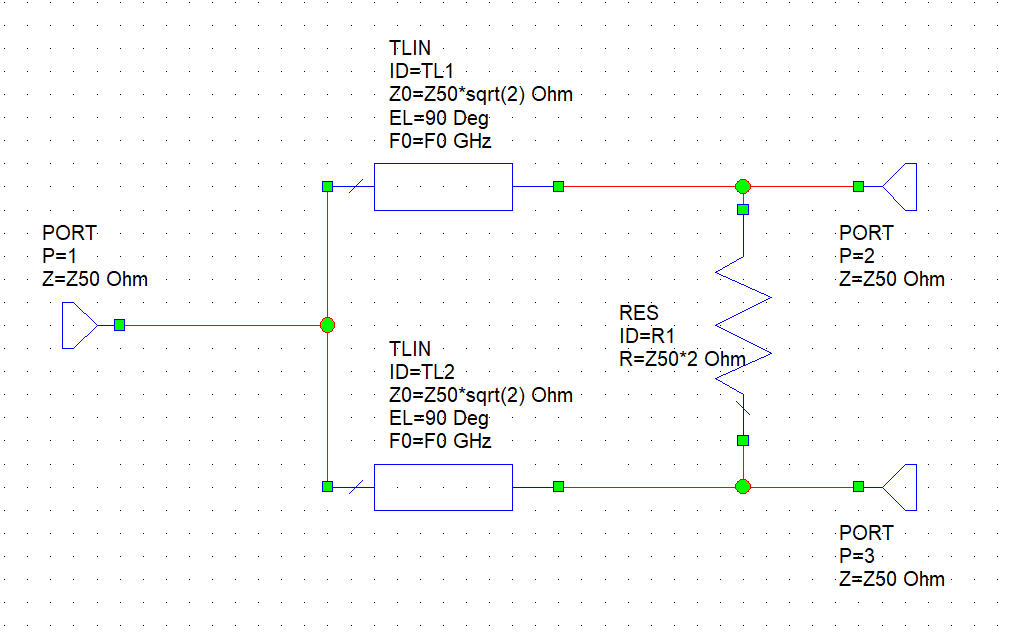
\includegraphics[width=\linewidth]{images/microstrip_elements/wilkinson_ideal_circuit.png}
    \caption{Ideal Wilkinson power divider / combiner circuit}
    \label{fig:microstrip_elements:wilkinson_ideal_circuit}
\end{figure}

If we simulate the circuit of Figure \ref{fig:microstrip_elements:wilkinson_ideal_circuit}, we get the following graph (see Figure \ref{fig:microstrip_elements:wilkinson_ideal_graph}). Here we can see that the reflected power is 0 as $s_{11} = - 249 dB$. And the transmitted power for each port is $s_{21} = s_{31} = 3 \ dB = 0.5$, that is half of the input power goes to each port.

\begin{figure}[htbp]
    \centering
    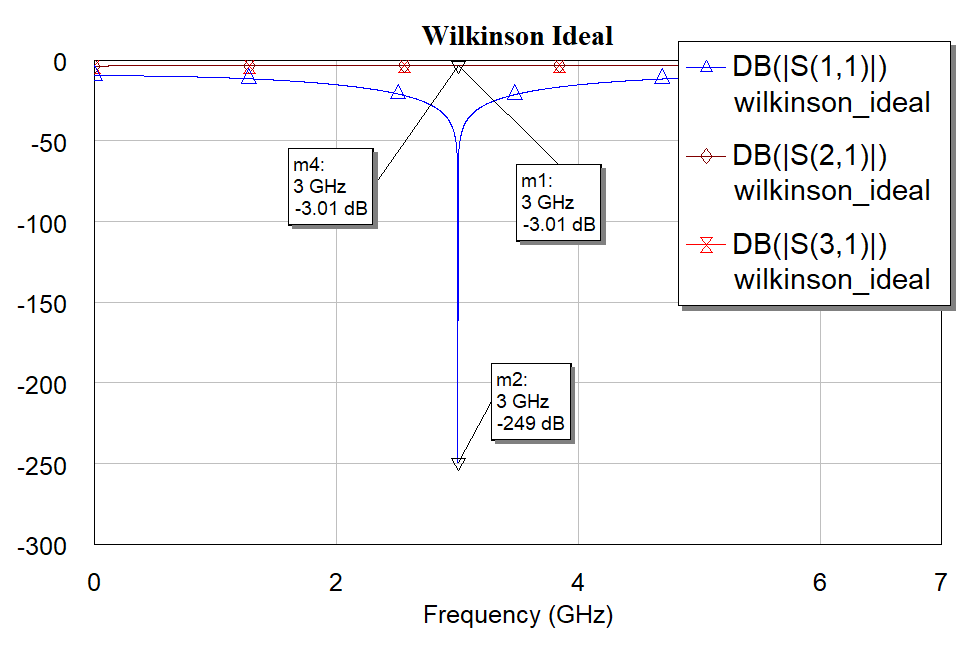
\includegraphics[width=1\linewidth]{images//microstrip_elements/wilkinson_ideal_graph.png}
    \caption{Simulation of an ideal Wilkinson power divider / combiner}
    \label{fig:microstrip_elements:wilkinson_ideal_graph}
\end{figure}

\subsection{Implementation with transmission lines}

In order to implement this in our design, we will have to adapt the ideal Wilkinson power divider / combiner to our circuit. For this we will have to calculate the width and length of the TLs for a characteristic impedance of $Z_{0,W} = 70.71 \ \Omega$. For this we have used the TXLine tool of AWR and we got a width of $w = 0.9065 mm$ and a height of $h = 12.19 mm$ (see Figure \ref{fig:microstrip_elements:wilkinson_real_txline_tool_calculations}).

\begin{figure}[htbp]
    \centering
    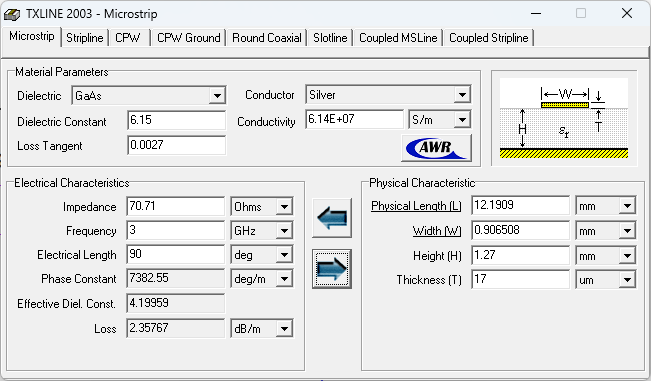
\includegraphics[width=1\linewidth]{images//microstrip_elements/wilkinson_real_txline_tool_calculations.png}
    \caption{Calculations of the width and height of the Wilkinson power divider / combiner}
    \label{fig:microstrip_elements:wilkinson_real_txline_tool_calculations}
\end{figure}

Now, if we simulate the following circuit with the TL with the correct dimensions (see Figure \ref{fig:microstrip_elements:wilkinson_real_circuit}), we get the graph shown in Figure \ref{fig:microstrip_elements:wilkinson_real_graph}.
Here we can observe that the implementation of the Wilkinson power divider / combiner works correctly as it divides the power in half and it has almost no reflection. However, this implementation is really difficult to implement in a microstrip line, so let's change the design to make it easier to implement.

\begin{figure}[htbp]
    \centering
    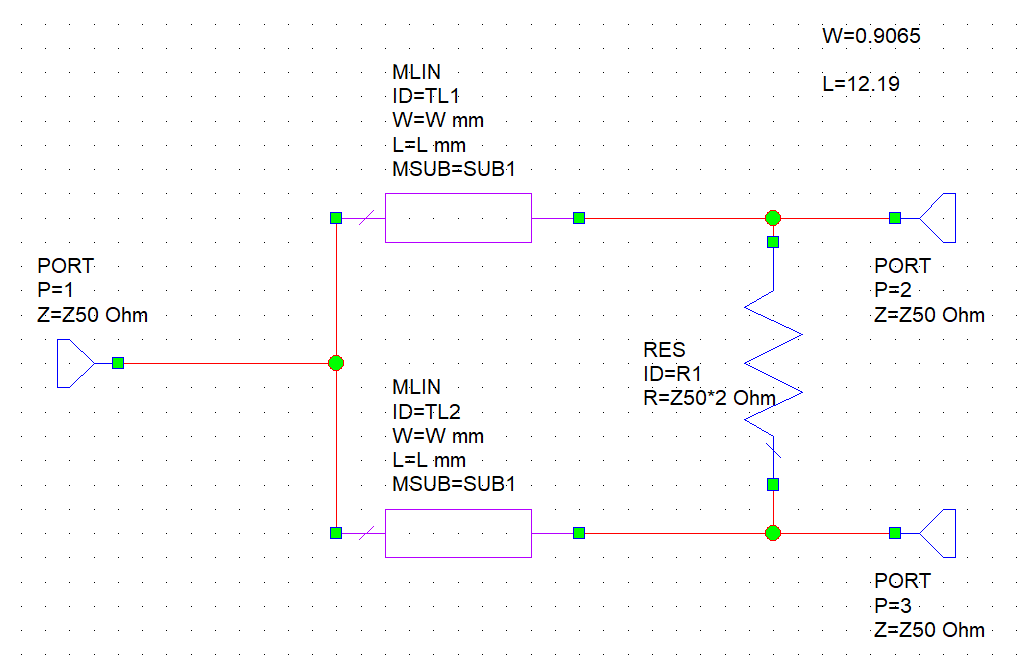
\includegraphics[width=1\linewidth]{images//microstrip_elements/wilkinson_real_circuit.png}
    \caption{Microstrip circuit design of the Wilkinson power divider / combiner}
    \label{fig:microstrip_elements:wilkinson_real_circuit}
\end{figure}

\begin{figure}[htbp]
    \centering
    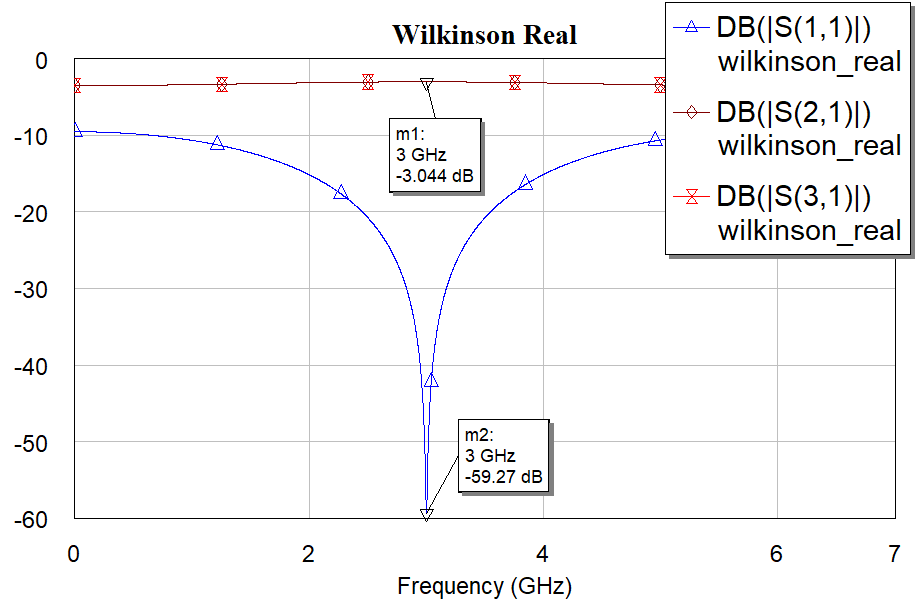
\includegraphics[width=1\linewidth]{images//microstrip_elements/wilkinson_real_graph.png}
    \caption{Simulation of the real Wilkinson power divider / combiner}
    \label{fig:microstrip_elements:wilkinson_real_graph}
\end{figure}

\subsection{Implementation with TEE junctions}

In order to incorporate the Wilkinson power divider / combiner in a microstrip technology, we will be using TEE junctions as \question{why is it better?}. For this implementation we will have to calculate the different radius shown in Figure \ref{fig:microstrip_elements:wilkinson_tee_design}. Note that the Gap will be the one required to solder the 0603 SMD resistor, for our case, we will be using $Gap = 1 mm$.

\begin{figure}
    \centering
    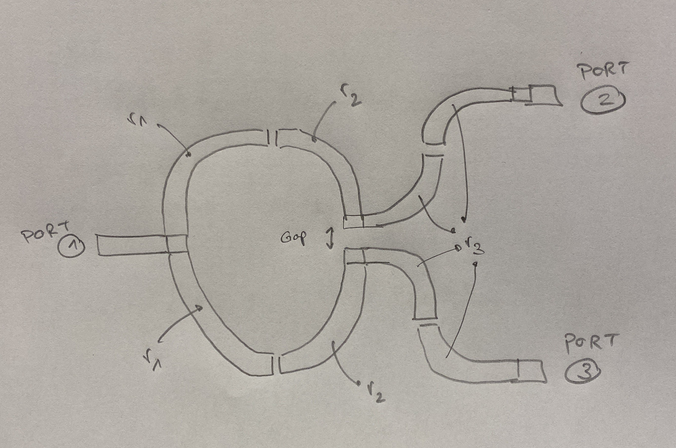
\includegraphics[width=1\linewidth]{images//microstrip_elements/wilkinson_tee_design.png}
    \caption{Design for the implementation of a Wilkinson with TEE junctions}
    \label{fig:microstrip_elements:wilkinson_tee_design}
\end{figure}

\begin{align*}
    r_1 &= \frac{1}{2} \* (\frac{\lambda}{2 \* \pi} + \frac{W_{50} + Gap}{2})  = \frac{1}{2} \* (\frac{c}{2 \* \pi \* f \* \sqrt{\epsilon_r}} + \frac{W_{50} + Gap}{2})  \\
    &= \frac{1}{2} \* (\frac{3 \cdot 10^8}{2 \* \pi \* 3 \cdot 10^9 \* \sqrt{6.15}} + \frac{1.85 \cdot 10^{-3} + 1 \cdot 10^{-3}}{2})  \\
    &= 4.031 \cdot 10^{-3} m = 4.031 mm \\
    \\
    r_2 &= r_1 - \frac{W_{50} + Gap}{2}  \\
    &= 4.031 \cdot 10^{-3} - \frac{1.85 \cdot 10^{-3} + 1 \cdot 10^{-3}}{2}  \\
    &= 2.606 \cdot 10^{-3} m = 2.606 mm \\
    \\
    r_3 &= \frac{\lambda}{2} = \frac{c}{f \* \sqrt{\epsilon_r}} \\
    &= \frac{3 \cdot 10^8}{3 \cdot 10^9 \* \sqrt{6.15}} \\
    &= 0.04032 m = 40.32 mm \\
\end{align*}

Note: the width, $W_{50} = 1.85 mm$, we use is the one calculated in Figure \ref{fig:previous_work:duroid_6006_h_1_27_mm_50_ohm}.

\todo{add circuit, graph and layout}

\section{First Stage: Simple Amplifier}


\subsection{Wideband Simulation of the Vendor's Bias Network}

\question{Simulation done but I have a question on the length of the TLs (Andres)}

\subsection{Wideband Simulation of the Proposed Bias Network}

\question{Simulation done but I have a question on the length of the TLs (Andres)}


\section{Second Stage: Balanced Amplifier}
\section{Band Pass Filter}

\section{Directional Coupler}

For the directional coupler, in order to adapt the ideal directional coupler of Figure \ref{fig:design_circuit_elements:directional_coupler_ideal_circuit}, we need to calculate the parameters of the microstrip line.

\subsection{Calculation of the length, width, and separation of the coupled microstrip lines}

In order to calculate the, we used the Tunner Tool of AWR where we modified the length (L), width (W), and separation (S) until we got a coupling of $C = 20 \ dB$ and a reflected power of as low as possible. For this simulation we have used the circuit pictured in Figure .

\question{how to tune it properly, i dont get a good value}






%-------------------------------------
\chapter{Integration}

\section{Common Microstrip Layout}

\section{Simulation of the Full Network at Working Frequencies}

\section{Matching Networks} % Maybe it is not necessary

\section{Simulation of the Full Network Wideband Response (0GHz up to 7GHz}







%-------------------------------------
\chapter{Results and Conclusions}

\section{Comparison of the System Specifications with the Simulated Results}

\section{Conclusions} % where you justify your design decisions, and any possible specifications that are not fulfilled, and also the critical aspects of the design.
























%----------
%	BIBLIOGRAFÍA
%----------	

%\nocite{*} % Si quieres que aparezcan en la bibliografía todos los documentos que la componen (también los que no estén citados en el texto) descomenta está línea

\clearpage
\addcontentsline{toc}{chapter}{Bibliografía}
%\setquotestyle[english]{british} % Cambiamos el tipo de cita porque en el estilo IEEE se usan las comillas inglesas.
\printbibliography


%----------
%	ANEXOS
%----------	

% Si tu trabajo incluye anexos, puedes descomentar las siguientes líneas
%\chapter* {Anexo x}
%\pagenumbering{gobble} % Las páginas de los anexos no se numeran



\end{document}